\documentclass[12pt]{article}
\usepackage[utf8]{inputenc}
\usepackage{graphicx}
\graphicspath{ {./images/} }
\usepackage{subcaption}
\usepackage{float}


\begin{document}
\begin{titlepage}
\newcommand{\HRule}{\rule{\linewidth}{0.1mm}} 
\center

\textsc{\Large CSE 421}\\[0.5cm] 
\textsc{\Large Artificial Intelligence}\\[0.5cm]
\textsc{\large Report On }\\[0.5cm] 

\HRule \\[0.4cm]
{ \huge \bfseries Shape and Material from Sound}\\[0.1cm] 
\HRule \\[1.5cm]
 

\begin{minipage}{0.4\textwidth}
\begin{flushleft} \large

\emph{Submitted By:}\\
Prerana \textsc{Das}\\
ID:161-115-119 \\ 
Session:2016-2019 \\
Batch: 38th\\
Section: C\\
\end{flushleft}
 


\end{minipage}
\begin{minipage}{0.4\textwidth}
\begin{flushright} \large
\emph{Instructor:} \\
Arif \textsc{Ahmed}\\ % Instructor's Name
Senior \textsc{Lecturer}\\
Dept. of CSE\\
\end{flushright}
\end{minipage}\\[1cm]

 

{\large \today}\\[1cm] % Date, change the \today to a set date if you want to be precise

\includegraphics{logo.png}% \\[0.5cm] % 
\vfill % Fill the rest of the page with white-space

\end{titlepage}

\tableofcontents       
\listoffigures
\thispagestyle{empty}

\section{Introduction}
\subsection{Main Idea}
When One object fall onto the ground it's makes a sound. By hearing this sound any 
human being can predict this object shape material and falling height. Because one human being has unknown capacity of knowledge.So at a short period of time they can make a big amount of information.\\
In this paper they build such a machine to predict all of this properties.
\begin{itemize} 
\item Estimate physical properties of the objects
\item Compare this predictions with human response
\item The developed model makes to some real data
\item The model achieves near-human performance

\end{itemize}


\subsection{Contribution}
Build a machine which can infer raw shapes, materials and falling height of an object from sound.\\
First of all we collect a set of human knowledge for an falling object by the help of physics based simulation engine. Also use analysis by synthesis approach to infer properties.
Then map their prediction with previous information.


\section{Major Experimental Results}
Construct an audio dataset that includes 14 primitives .Each with 10 different moduli.\\
\\
\begin{tabular}{|l|l|l|l}
\hline
Variable & Range & C/T\\
\hline
Primtive Shape(s) & 14 classes & D \\
Height (z) & [1, 2] & C\\
Rotation axis (i, j, k) & S2 & C\\
Rayleigh damping $(\alpha)$ & $10[-8,-5]$ & C\\
Specific modulus $(E/\rho)$ & $[1, 30] \times 106$ & D\\
Restitution (e) & [0.6, 0.9] & C\\
Rotation angle (w) & $[-\pi, \pi)$ & C\\
Rayleigh damping $(\beta)$ & 2[0,5] & C\\
\hline
\end{tabular} 
\\
\\
Initial and final classification accuracies and parameter MSE errors of three different inference models after 80 iteration of MCMC are showing below. 
\\
\\
% -----Gibbs sampling
\textbf{Gibbs sampling} \newline  \newline
1. Begin with some initial value  $ {X} ^{(i)} $ 
\newline \newline
2.We want the next sample. Call this next sample $ {X} ^{(i+1)} =  ( {X} ^{(i+1)} , {X} ^{(i+2)}, .... {X} ^{(i+n)}) $ \newline \newline
3.Update it according to the distribution specified by $ {X}_j
^{(i+1)} | ( {X}_1 ^{(i+1)} ,... {X}_j-1
^{(i+1)},{X}_j+1
^{(i)} .... {X}_n ^{(i)}) $ \newline \newline

\section{Strength And Weaknesses}
% -----Strength
\subsubsection{Strength}
No need to visual perception.Three binary judgemental about the shape by listening to our synthesized audio clip. Humans are relatively good at recognizing shape attributes from sound. From a audio clips we get some physical properties those are density young's modulus and damping coefficients.
This model also can measure falling height whether an object dropped from to the ground. Find out the sence setup . 
% -----Weaknesses
\subsubsection{Weaknesses}
For inferring materials from sound let one physical objects property has four possible materials those are steel, ceramic, polystyrene and wood.There should be choose one out of four parameter.However sometimes this is to much difficult when sampled ones have similar damping and specific modulus.\\
This machine confused steel with ceramic and ceramic with polystyrene. This is the greatest weakness in this inference model.

% -----follow-up work
\section{Follow-up Works}

For sound wave simulator. This simulation lets you see the movement of a sound wave. Adjust the frequency and can see and hear how the wave change.
\newline
\newline
\subsection{Unsupervised}
Recover the latent variables x to make the reproduced sound.
Use the spectrogram as a feature and measure the
$ l_{2} $ distance between the spectrograms of two sounds, because Young’s modulus will only affect the
frequency at each collision

\subsection{Self-supervised Learning}
\begin{itemize} 
\item Train a deep neural network
\item Limited number of iterations
\item Runs analysis-by-synthesis algorithm to refine the inference
\end{itemize} 

\subsection{Weakly-supervised Learning}
\begin{itemize} 
\item It is more realistic to assume
\item Limited number of data that easy to get
\item Refer to learning with noisy labels
\end{itemize}

\subsection{Fully-supervised Learning}
\begin{itemize} 
\item To visualize the abstraction and characteristic features
\item Inputs maximally activated
\end{itemize}

$ Sound Synthesis \rightarrow Sound Propagation \rightarrow Sound Rendering $
\\
\\
\\
\textsc{\Large List of Figure }\\[0.5cm] 

\begin{figure}[H]
	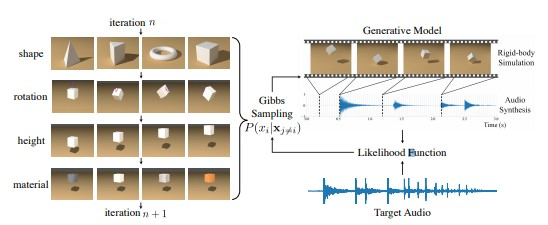
\includegraphics[width=16cm, height=6cm]{fig1.jpg}
	\caption{Our inference pipeline. We use Gibbs sampling over the latent variables. The conditional
probability is approximated using the likelihood between reconstructed sound and the input sound}
	\label{fig:fig1} 	
\end{figure}

\begin{figure}[H]
	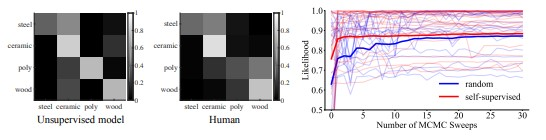
\includegraphics[width=16cm, height=6cm]{fig2.jpg}
	\caption{Left and middle: confusion matrix of material classification performed by human and our
unsupervised model. Right: mean likelihood curve over MCMC iterations}
	\label{fig:fig2} 	
\end{figure}

\begin{figure}[H]
	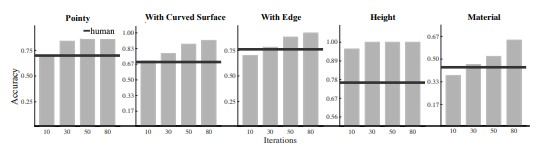
\includegraphics[width=16cm, height=6cm]{fig3.jpg}
	\caption{Human performance and unsupervised performance comparison. The horizontal line
represents human performance for each task. Our algorithm closely matches human performance}
	\label{fig:fig3} 	
\end{figure}

\begin{figure}[H]
	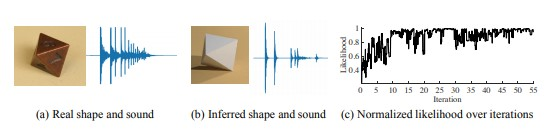
\includegraphics[width=16cm, height=6cm]{fig4.jpg}
	\caption{Results of inference on real world data. The test recording is made by dropping the metal
dice in (a). Our inferred shape and reproduced sound is shown in (b). Likelihood over iteration is
plotted in (c)}
	\label{fig:fig4} 	
\end{figure}


\cite{gratzer2007more}

\bibliographystyle{plain}
\bibliography{Bibliography.bib} 

\end{document}

